\documentclass[border=5pt]{standalone}
\usepackage{pgfplots}
\pgfplotsset{compat=1.18}
\usepgfplotslibrary{statistics}

\begin{document}
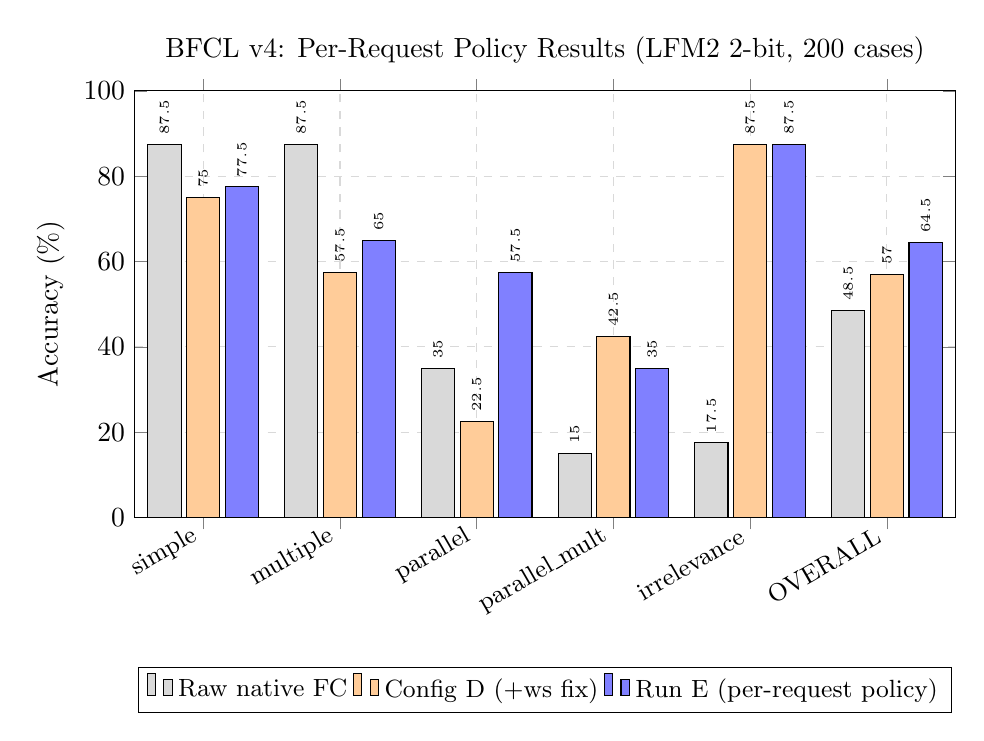
\begin{tikzpicture}
\begin{axis}[
    ybar,
    bar width=12pt,
    width=12cm,
    height=7cm,
    ylabel={Accuracy (\%)},
    symbolic x coords={simple, multiple, parallel, parallel\_mult, irrelevance, OVERALL},
    xtick=data,
    x tick label style={rotate=30, anchor=east, font=\small},
    ymin=0, ymax=100,
    legend style={at={(0.5,-0.35)}, anchor=north, legend columns=3, font=\small},
    nodes near coords,
    every node near coord/.append style={font=\tiny, rotate=90, anchor=west},
    grid=major,
    grid style={dashed, gray!30},
    title={BFCL v4: Per-Request Policy Results (LFM2 2-bit, 200 cases)},
]

% Raw native FC (baseline)
\addplot[fill=gray!30] coordinates {
    (simple, 87.5) (multiple, 87.5) (parallel, 35.0) (parallel\_mult, 15.0) (irrelevance, 17.5) (OVERALL, 48.5)
};

% Config D (whitespace fix)
\addplot[fill=orange!40] coordinates {
    (simple, 75.0) (multiple, 57.5) (parallel, 22.5) (parallel\_mult, 42.5) (irrelevance, 87.5) (OVERALL, 57.0)
};

% Run E (per-request policy, final)
\addplot[fill=blue!50] coordinates {
    (simple, 77.5) (multiple, 65.0) (parallel, 57.5) (parallel\_mult, 35.0) (irrelevance, 87.5) (OVERALL, 64.5)
};

\legend{Raw native FC, Config D (+ws fix), Run E (per-request policy)}

\end{axis}
\end{tikzpicture}
\end{document}
